\chapter{Задание}

Цель лабораторной работы: реализовать ПО, позволяющее по заданным параметрам построить графики функции распределения и плотности вероятности заданных распределений.

Для выполнения поставленной цели требуется:
\begin{itemize}
	\item привести формулы функции распределения и плотности вероятности заданных распределений;
	\item объяснить физический смысл распределений;
	\item написать программу на любом средстве реализации для решения поставленной цели;
	\item привести листинги кода и демонстрацию работы программы.
\end{itemize}

Мой вариант -- 3.
Согласно требованиям к лабораторной работе, нужно провести работу с двумя распределениями:
\begin{enumerate}
	\item Равномерное распределение.
	\item Распределение Эрланга.
\end{enumerate}

\chapter{Теоретическая часть}
В этом разделе будут рассмотрены два распределения: равномерное и Эрланга. Будут приведены их формулы плотности распределения и функции распределения, а также рассмотрен физический смысл распределений.
\section{Равномерное распределение}
\textbf{Равномерное распределение} -- распределение случайной величины, принимающей значения, принадлежащие некоторому промежутку конечной длины, характеризующееся тем, что плотность вероятности на этом промежутке постоянна.

Функция равномерного распределения:

\begin{equation}
    F_X(x) =
    \begin{cases}
            0, x < a, \\
            \begin{aligned}
                \frac{x -  a}{b - a}, x \in [a, b], 
            \end{aligned}\\
            0, x > b. \\
    \end{cases}
\end{equation}

Функция плотности равномерного распределения:

\begin{equation}
    f_X(x) =
    \begin{cases}
            \begin{aligned}
                \frac{1}{b - a}, x \in [a, b], 
            \end{aligned}\\
            0, else. \\
    \end{cases}
\end{equation}
\subsection*{Физический смысл равномерного распределения}
Равномерное распределение возникает в тех ситуациях, когда каждая реализация выборки равновероятна.
Например, молекулы во время хаотического движения могут равновероятно двигаться в любом существующем направлении.

Имея генератор равномерного распределения и зная функцию, обратную к функции распределения случайной величины, можно построить генератор выборки любого непрерывного распределения (не обязательно равномерного) с помощью метода обратного преобразования.

Существуют также частные преобразования, позволяющие на основе равномерного распределения получить случайные распределения другого вида. Так, например, для получения нормального распределения используется преобразование Бокса — Мюллера.
\section{Распределение Эрланга}
\textbf{Распределение Эрланга} -- частный случай Гамма-распределения, двухпараметрическое абсолютно непрерывное распределение, в котором параметр $k$ принимает целочисленное значение.

Функция распределения Эрланга:

\begin{equation}
    \begin{aligned}
        F_k(x) = 1 - e^{-\lambda \cdot x} \cdot \sum_{i = 1}^{k - 1} \frac{(\lambda \cdot x)^i}{i!}.
    \end{aligned}
\end{equation}


Функция плотности распределения Эрланга:

\begin{equation}
    \begin{aligned}
        f_k(x) = \frac{\lambda \cdot (\lambda \cdot x)^{k - 1}}{(k - 1)!} \cdot e^{-\lambda \cdot x}.
    \end{aligned}
\end{equation}

В данных формулах $\lambda$ и $k$ --- положительные параметры распределения $(\lambda \geq 0; k = 1, 2, ...)$; $x \geq 0$.
\subsection*{Физический смысл распределения}
Распределение Эрланга названо в честь математика Агнера Эрланга, впервые применившего его в задачах теории массового обслуживания и телефонии. 

Это распределение интенсивно применяется в задачах телекоммуникации для моделирования входящего потока вызовов. Оно может быть также использовано для описания изменения работоспособности элемента системы, не имеющего резерва. Модель, построенная на этом распределении является более адекватной для описания поведения системы, чем экспоненциальная модель и охватывает два этапа эксплуатации, например, этапы проработки и нормальной эксплуатации. 
\chapter{Практическая часть}
\section{Выбор средств разработки ПО}
В качестве языка программирования выбран Python. 

Это обусловлено тем, что имеет опыт разработки на данном языке, а также наличием библиотек, позволяющих настраивать построение графиков, требуемых для работы.
\section{Листинги программы}

В листинге \ref{lst:distribution} представлен класс $Distribution$, отвечающий за вычисление значений функций распределения и плотности распределения.

\begin{lstlisting}[label=lst:distribution, caption=class Distribution]
class Distribution:
    def uniformDistribution(self, a: float, b: float, x: float):
        if x < a: return 0
        elif x > b: return 1
        else: return (x - a) / (b - a)
    def uniformDistributionDensity(self, a: float, b: float, x: float):
        if a <= x <= b: return 1 / (b - a)
        else: return 0
    def erlangDistribution(self, k: int, l: float, x: float):
        return 1 - exp((-1) * l * x) * \
            sum([pow(l * x, i) / factorial(i) for i in range(k)])
    def erlangDistributionDensity(self, k: int, l: float, x: float):
        return exp((-1) * l * x) * l * pow(l * x, k - 1) / factorial(k - 1)
\end{lstlisting}

\section{Демонстрация работы программы}

На рисунке \ref{img:uniformDistr} -- \ref{img:uniformDistr1} представлены графики функции распределения и функции плотности распределения для равномерного распределения с другими заданными параметрами.


\begin{figure}[h]
    \centering
    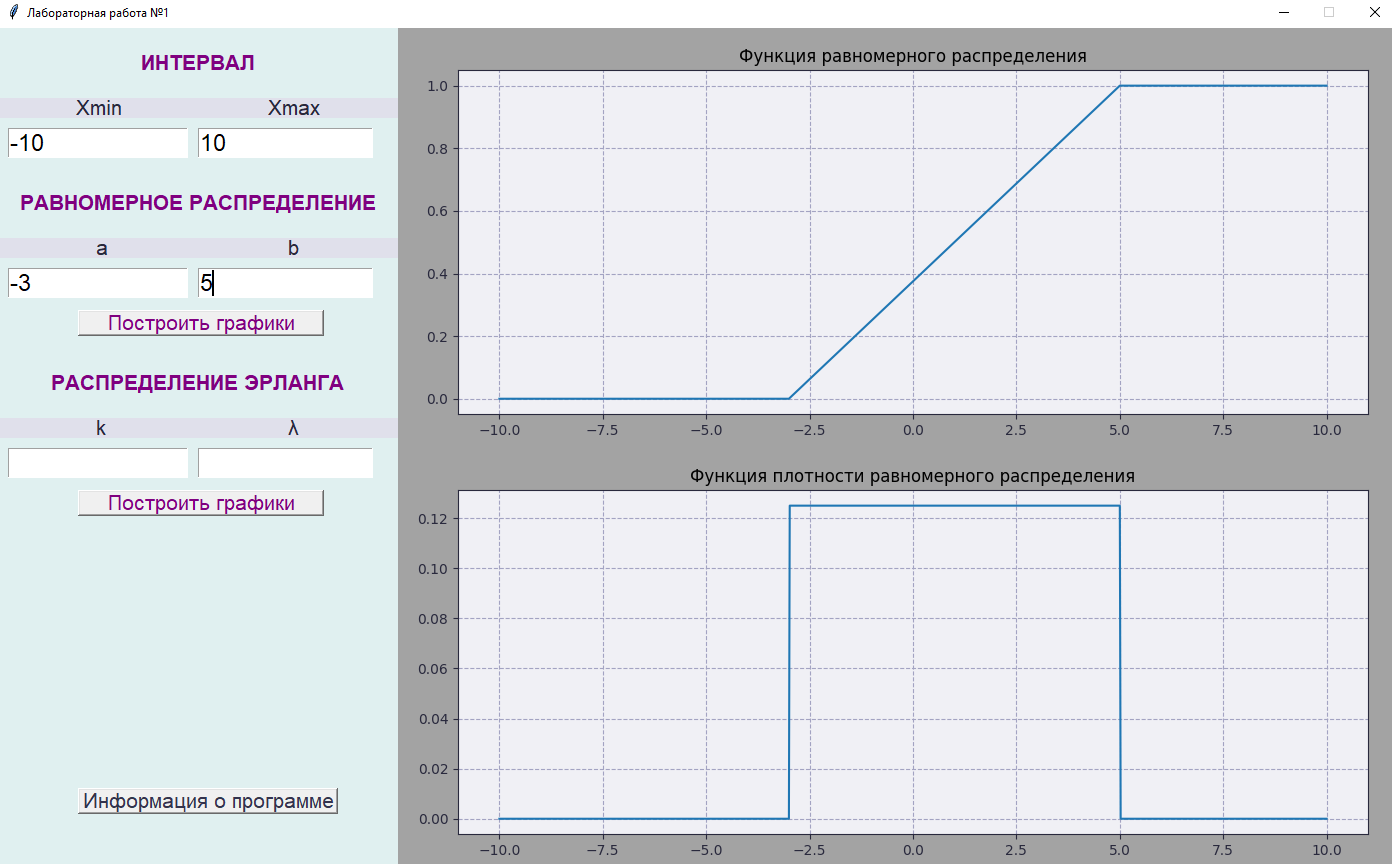
\includegraphics[scale = 0.44]{img/uniformDistr.png}
    \caption{Равномерное распределение}
    \label{img:uniformDistr}
\end{figure}
\clearpage
\begin{figure}[h]
    \centering
    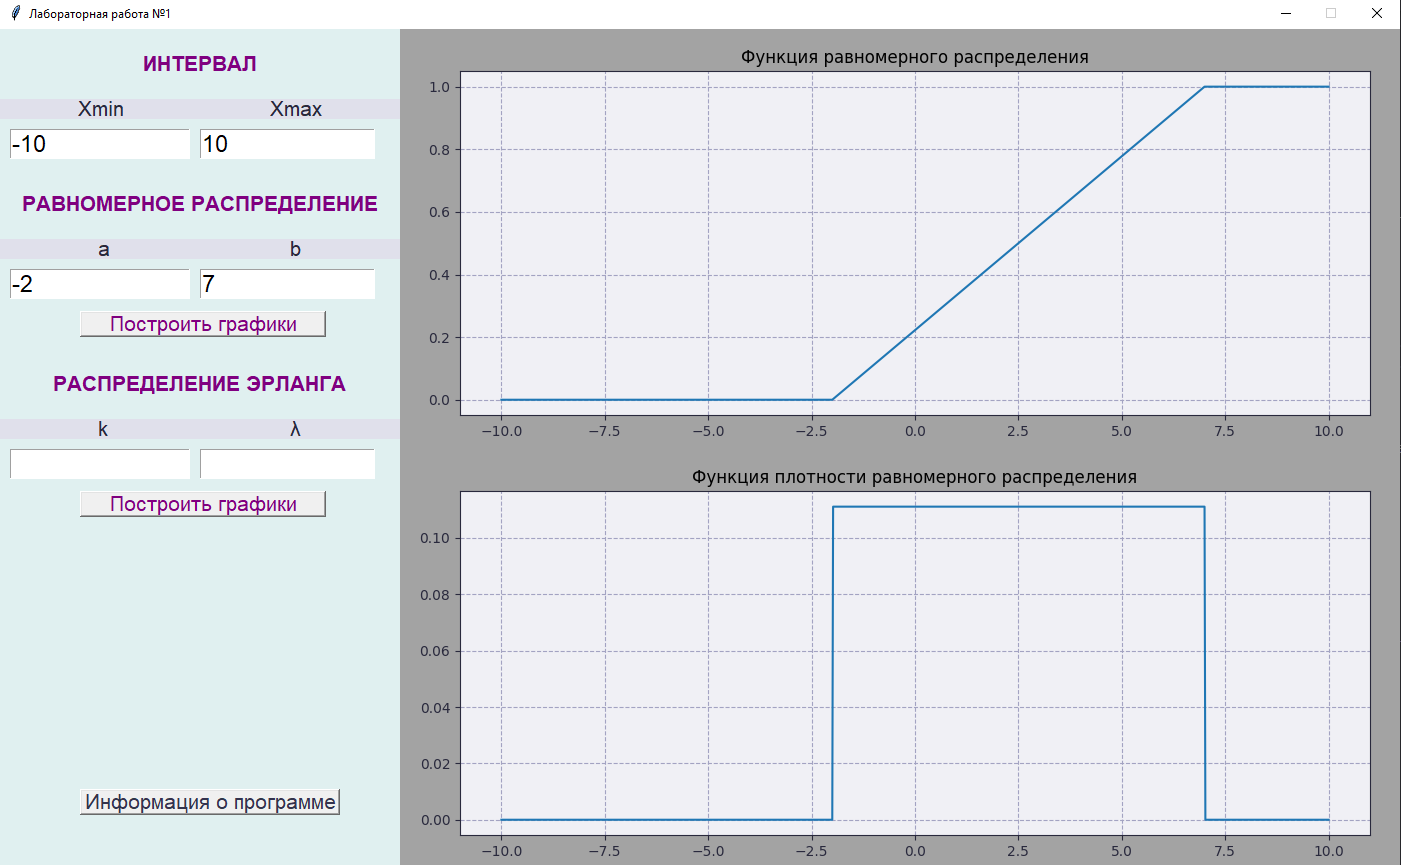
\includegraphics[scale = 0.44]{img/uniformDistr1.png}
    \caption{Равномерное распределение}
    \label{img:uniformDistr1}
\end{figure}

На рисунке \ref{img:erlangDistr} -- \ref{img:erlangDistr2} представлен график функции распределения и функции плотности распределения для распределения Эрланга с другими заданными параметрами.

\begin{figure}[h]
    \centering
    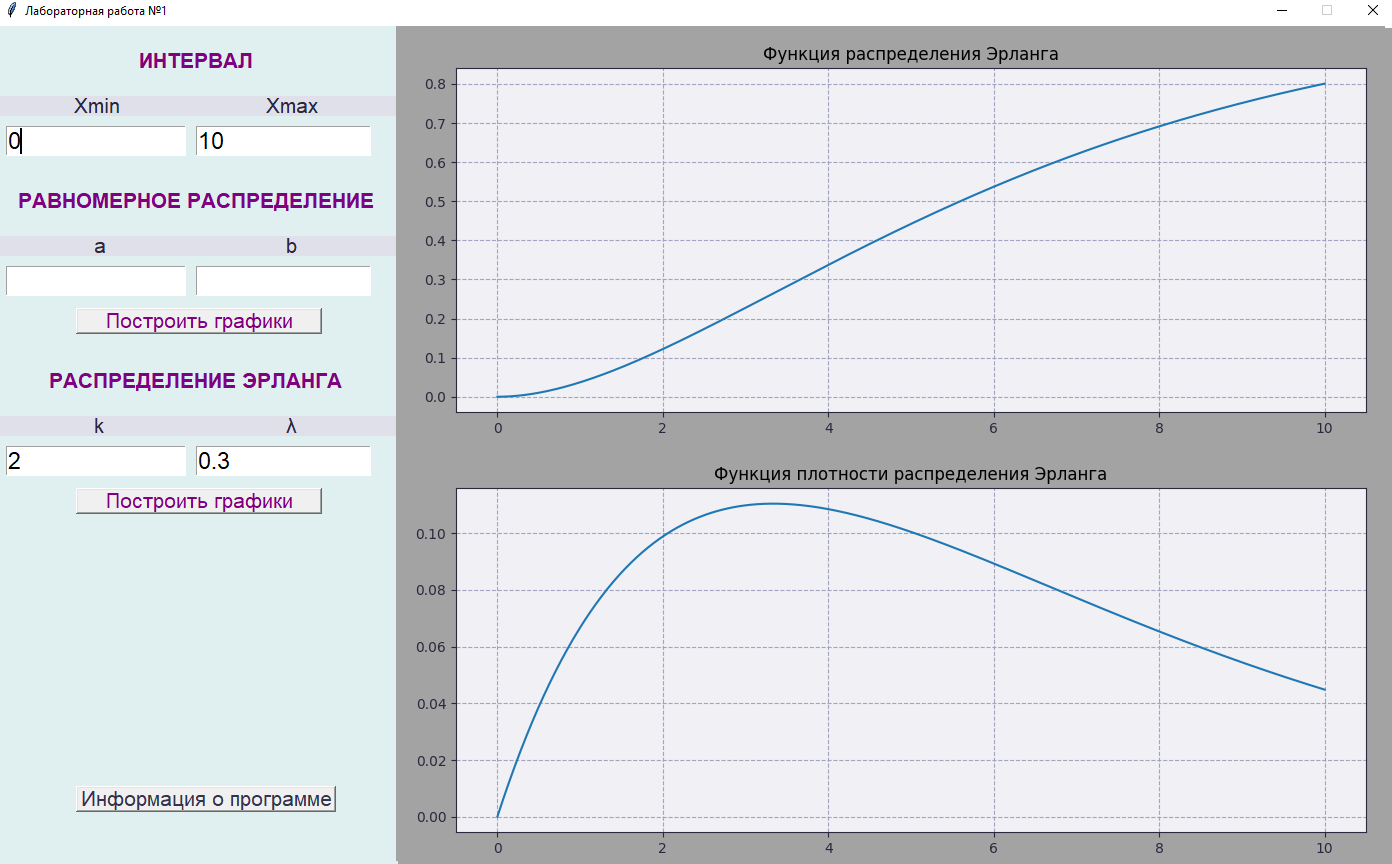
\includegraphics[scale=0.44]{img/erlangDistr.png}
    \caption{Распределение Эрланга}
    \label{img:erlangDistr}
\end{figure}

\begin{figure}[h]
    \centering
    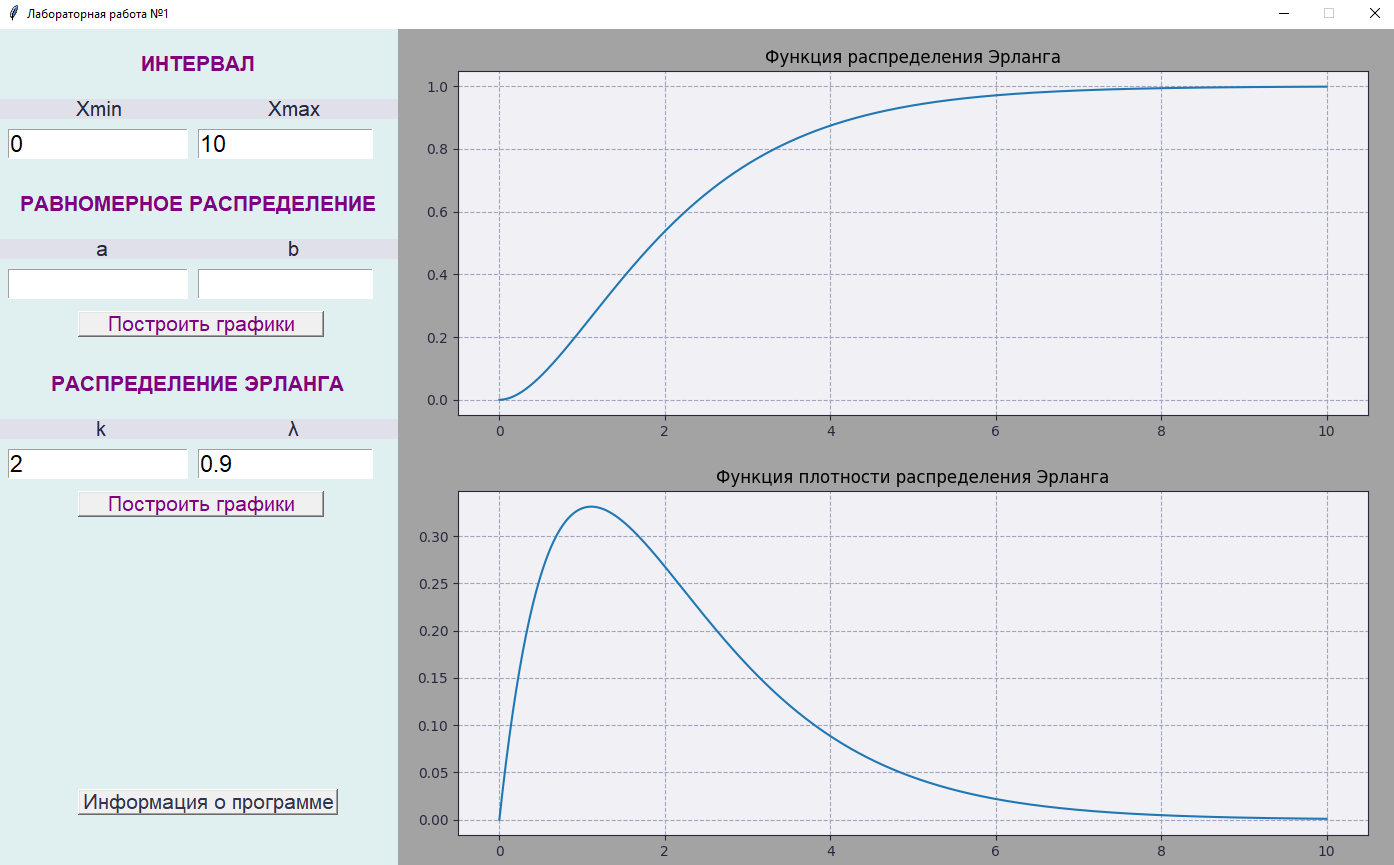
\includegraphics[scale=0.44]{img/erlangDistr1.png}
    \caption{Распределение Эрланга}
    \label{img:erlangDistr1}
\end{figure}

\begin{figure}[h]
    \centering
    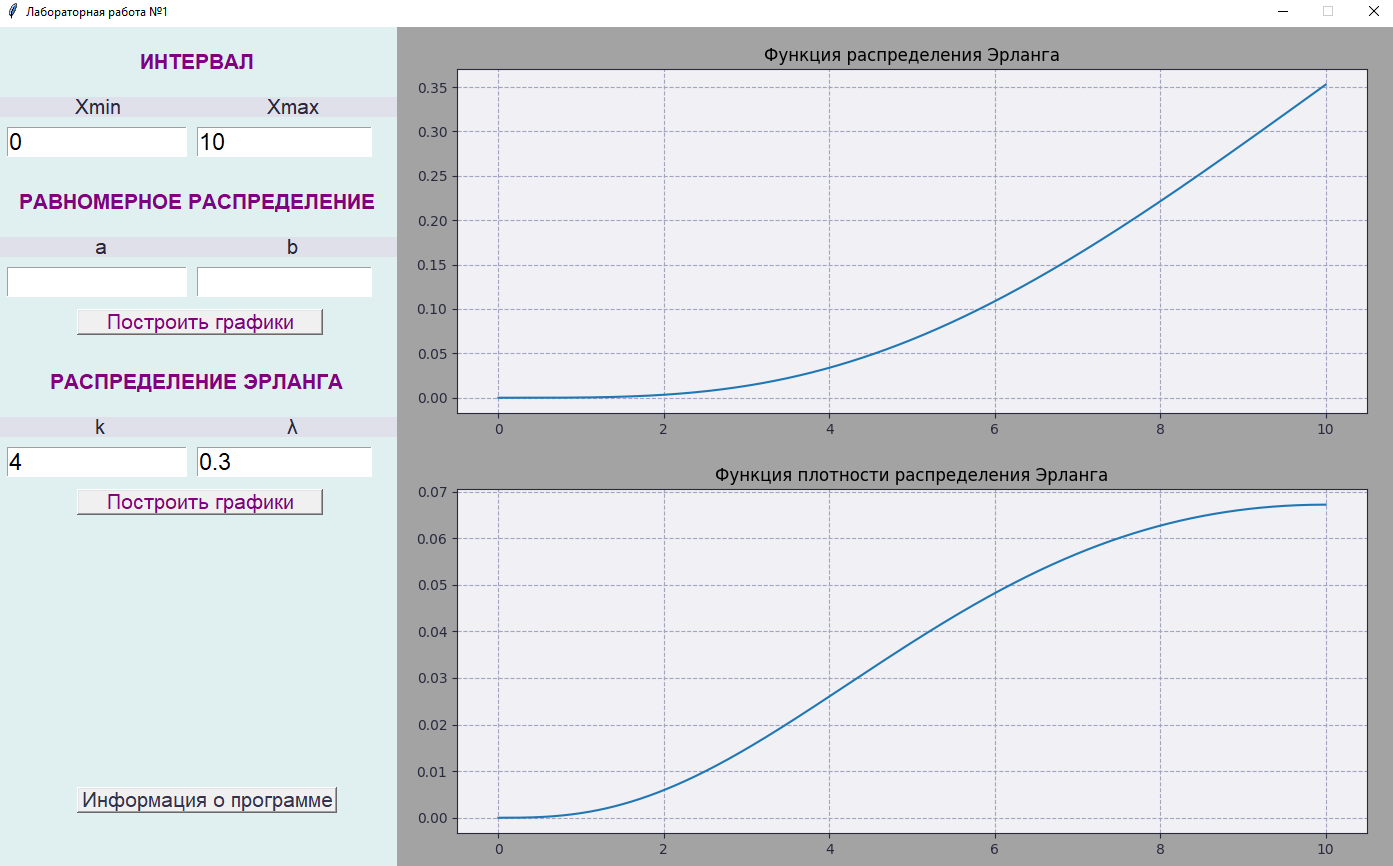
\includegraphics[scale=0.44]{img/erlangDistr2.png}
    \caption{Распределение Эрланга}
    \label{img:erlangDistr2}
\end{figure}